\begin{frame}		
	
	\frametitle{ARQ}
	\framesubtitle{Frame Timing}
	
	\begin{figure}[H]
		\center{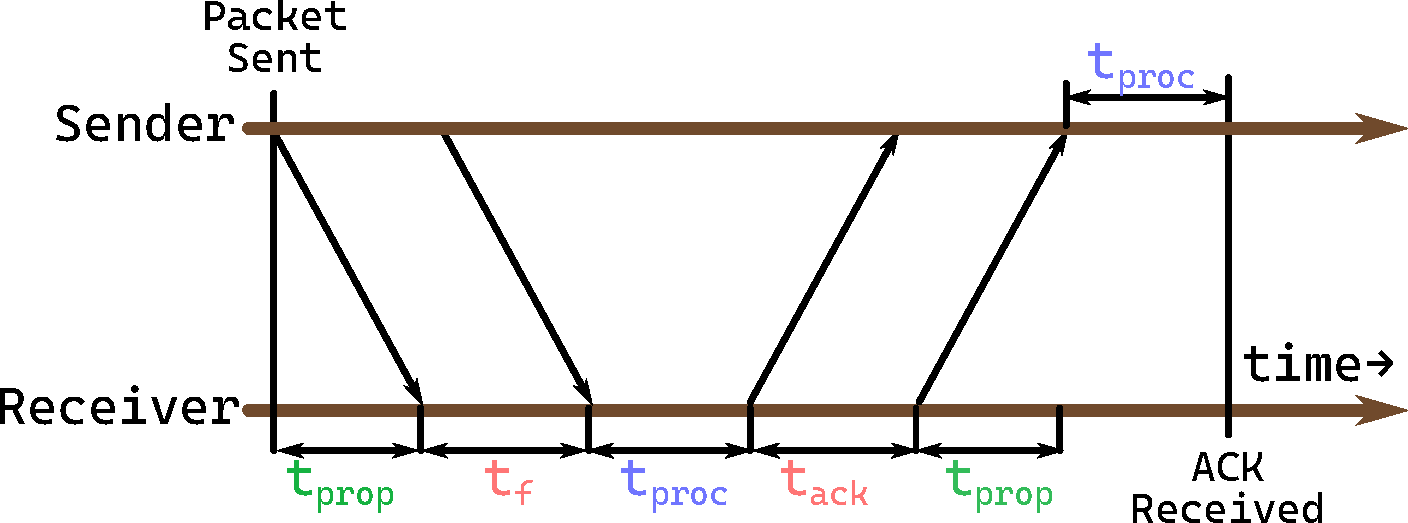
\includegraphics[width = 1\textwidth]{time}}
	\end{figure}
	
	$$t_0 = 2t_{prop} + t_f + 2t_{proc} + t_{ack} \approx RTT + 2t_{proc} + \dfrac{n_f + n_{ack}}{Rate}$$
	
\end{frame}

\begin{frame}		
	\frametitle{ARQ}
	\framesubtitle{Timing}
	
	
	\begin{itemize}
		\item Which timeout should we choose?
		\begin{itemize}
			\item Not too big
			\item Not too small
		\end{itemize}
		\item Easy to define for specific LAN. Little variation. 
		\item Difficult over the Internet. High variation.
	\end{itemize}
	
	
\end{frame}


\begin{frame}		
	\frametitle{ARQ}
	\framesubtitle{Adaptive Timeout}
	
	Simple Timeout calculation scheme\footnotemark[1]. Smoothed RTT + variance.
	
	\begin{itemize}
		\item $SRTT_{N+1} = 0.9 \cdot SRTT_N + 0.1 \cdot RTT_{N+1}$
		\item $Svar_{N+1} = 0.9 \cdot Svar_N = 0.1 \cdot |RTT_{N+1} - SRTT_{N+1}|$
		\item $Timeout_N = SRTT_N + 4 \cdot Svar_N$
	\end{itemize}
	\footnotetext[1]{\href{https://datatracker.ietf.org/doc/html/rfc2988}{rfc2988}}
\end{frame}

\begin{frame}		
	\frametitle{ARQ}
	\framesubtitle{Adaptive Timeout}
	
	\begin{figure}[H]
		\center{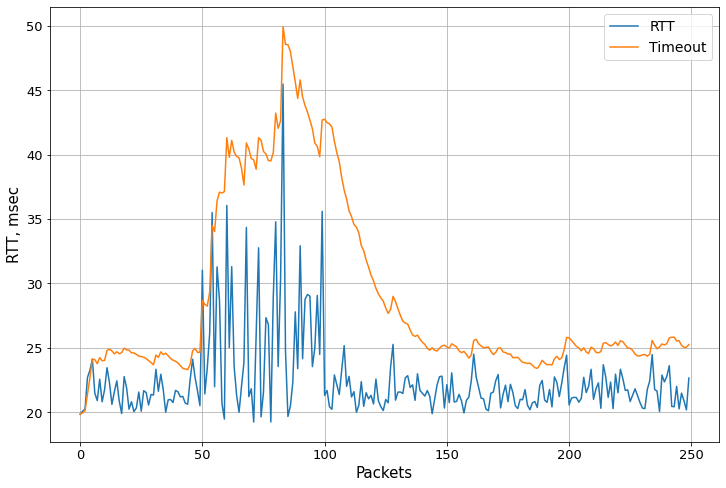
\includegraphics[width = 0.95\textwidth]{timeout_adaptive}}
	\end{figure}

\end{frame}